\chapter{Design Overview}

\section{General Design}

When developing this application, the user experience was at the forefront of my mind, guiding my design decisions.

I decided to design my application as a tab-based application, ensuring straightforward navigation and user-friendly interaction. This approach allows users to easily access different sections of the app, keeping the user experience organized and intuitive. I also decided to place a strong emphasis on minimalistic design principles to create an uncluttered and efficient interface. By stripping away unnecessary elements and focusing on essential functionalities, the app becomes user-centric and easy to use.

For the color scheme, shown in Figure \ref{fig:color-scheme}, I drew inspiration from the concept of cool colors. Cool colors, with their calming and relaxing properties, are chosen to evoke a sense of tranquility and ease within the app, ensuring users feel at ease and comfortable during their interaction with the platform \cite{Bilucaglia}.

\begin{figure}[H]
    \centering
    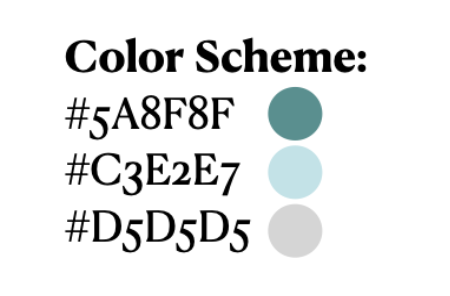
\includegraphics[width=0.2\linewidth]{thesis//chapters//images/colorScheme.png}
    \caption{Color Scheme}
    \label{fig:color-scheme}
\end{figure}

In addition, I aim to provide a design that is inclusive and accessible to all users. To achieve this, I carefully considered contrast and color choices, making sure they were tested against colorblind scales to ensure that the content was easily distinguishable and readable by a wide range of individuals.

To add a friendly and inviting touch to the app, I incorporated images and graphics that resonate with a warm and approachable feel. These images are thoughtfully chosen to create a connection with users and enhance their engagement with the app, contributing to a positive and enjoyable user experience.

In the following sections, you will see my initial prototype designs.

\section{Onboarding View}

The Onboarding Vew, shown in Figure \ref{fig:onboarding-screens}, consists of screens designed to introduce users to the app's key features and benefits. This view is essential for guiding new users and helping them get acquainted with the platform. The screens are simplistic and visually appealing, setting a positive tone for the user's journey.

The Set Up form asks the user to input key information, such as their name, birthdate, and allergens, and asks the user if they will allow the application to share data with Apple Health. This is a crucial step in the onboarding process, as without allowing access, the user will not have access to key insights and a tailored app experience.

\begin{figure}[H]
    \centering
    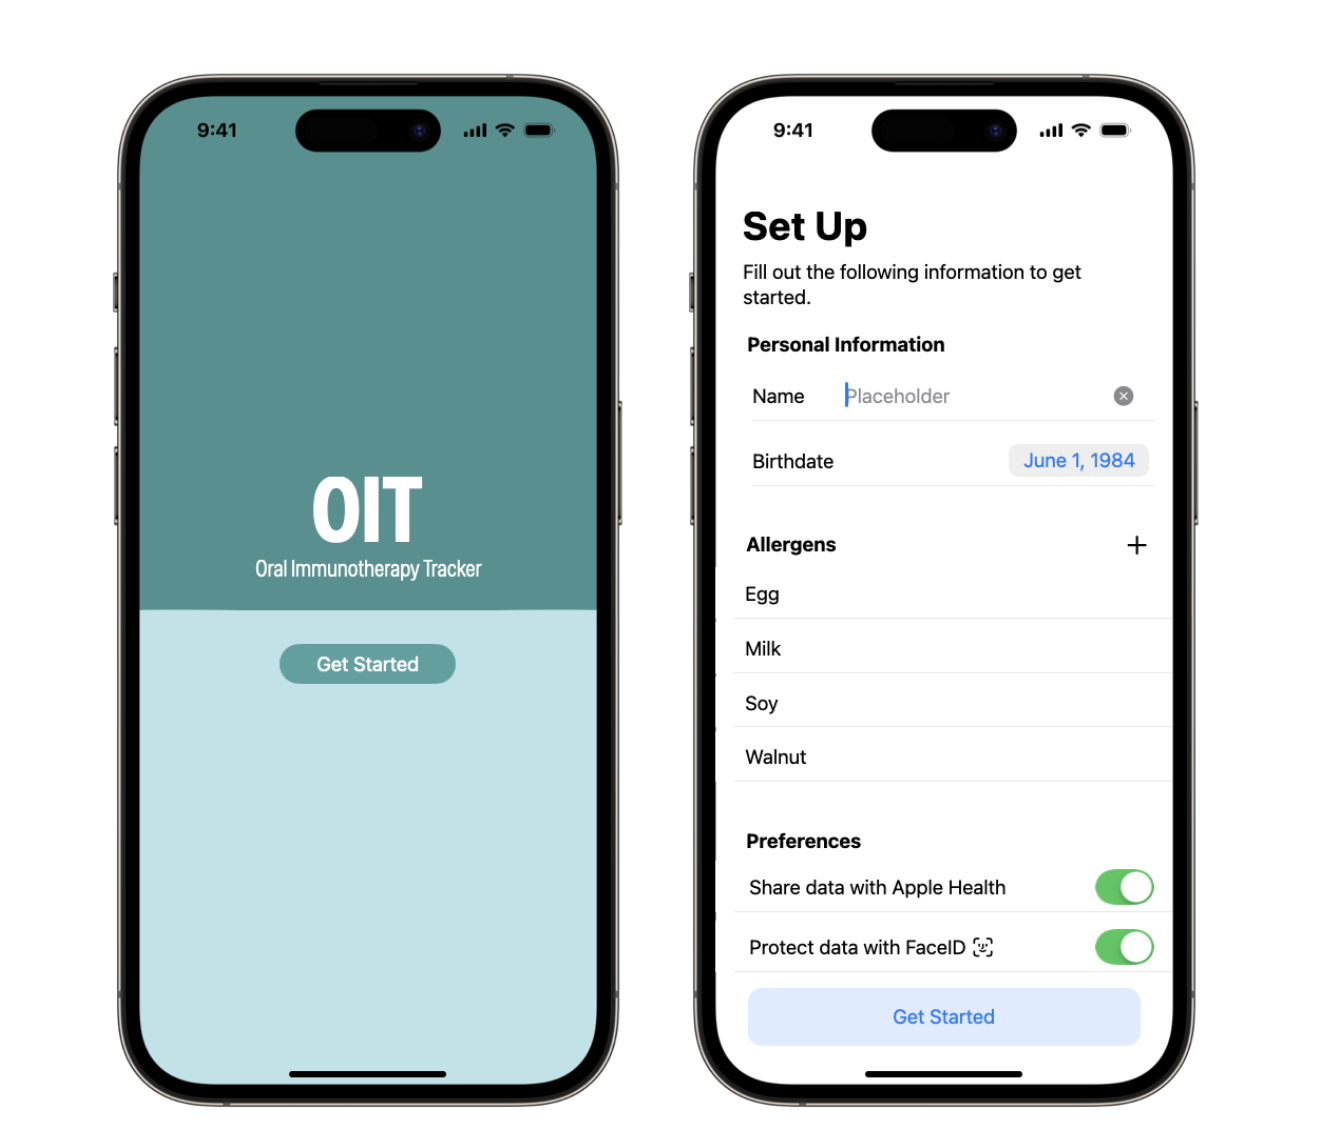
\includegraphics[width=0.5\linewidth]{thesis//chapters//images/onboarding-screens.png}
    \caption{Onboarding Screens}
    \label{fig:onboarding-screens}
\end{figure}

\section{Today Tab}

The Today Tab serves, shown in Figure \ref{fig:today-tab-screens}, as the core of the app, where users view and log dose and symptom information for the selected date. The design prioritizes clarity and easy navigation, ensuring users can quickly find the information they need. A sliding weekly calendar view allows the user to select a date, or the month button in the top right corner allows the user to switch to a monthly view. 

Additionally, the user can navigate to their profile from the Today Tab, where they can easily update their information, such as their allergens.

\begin{figure}[H]
    \centering
    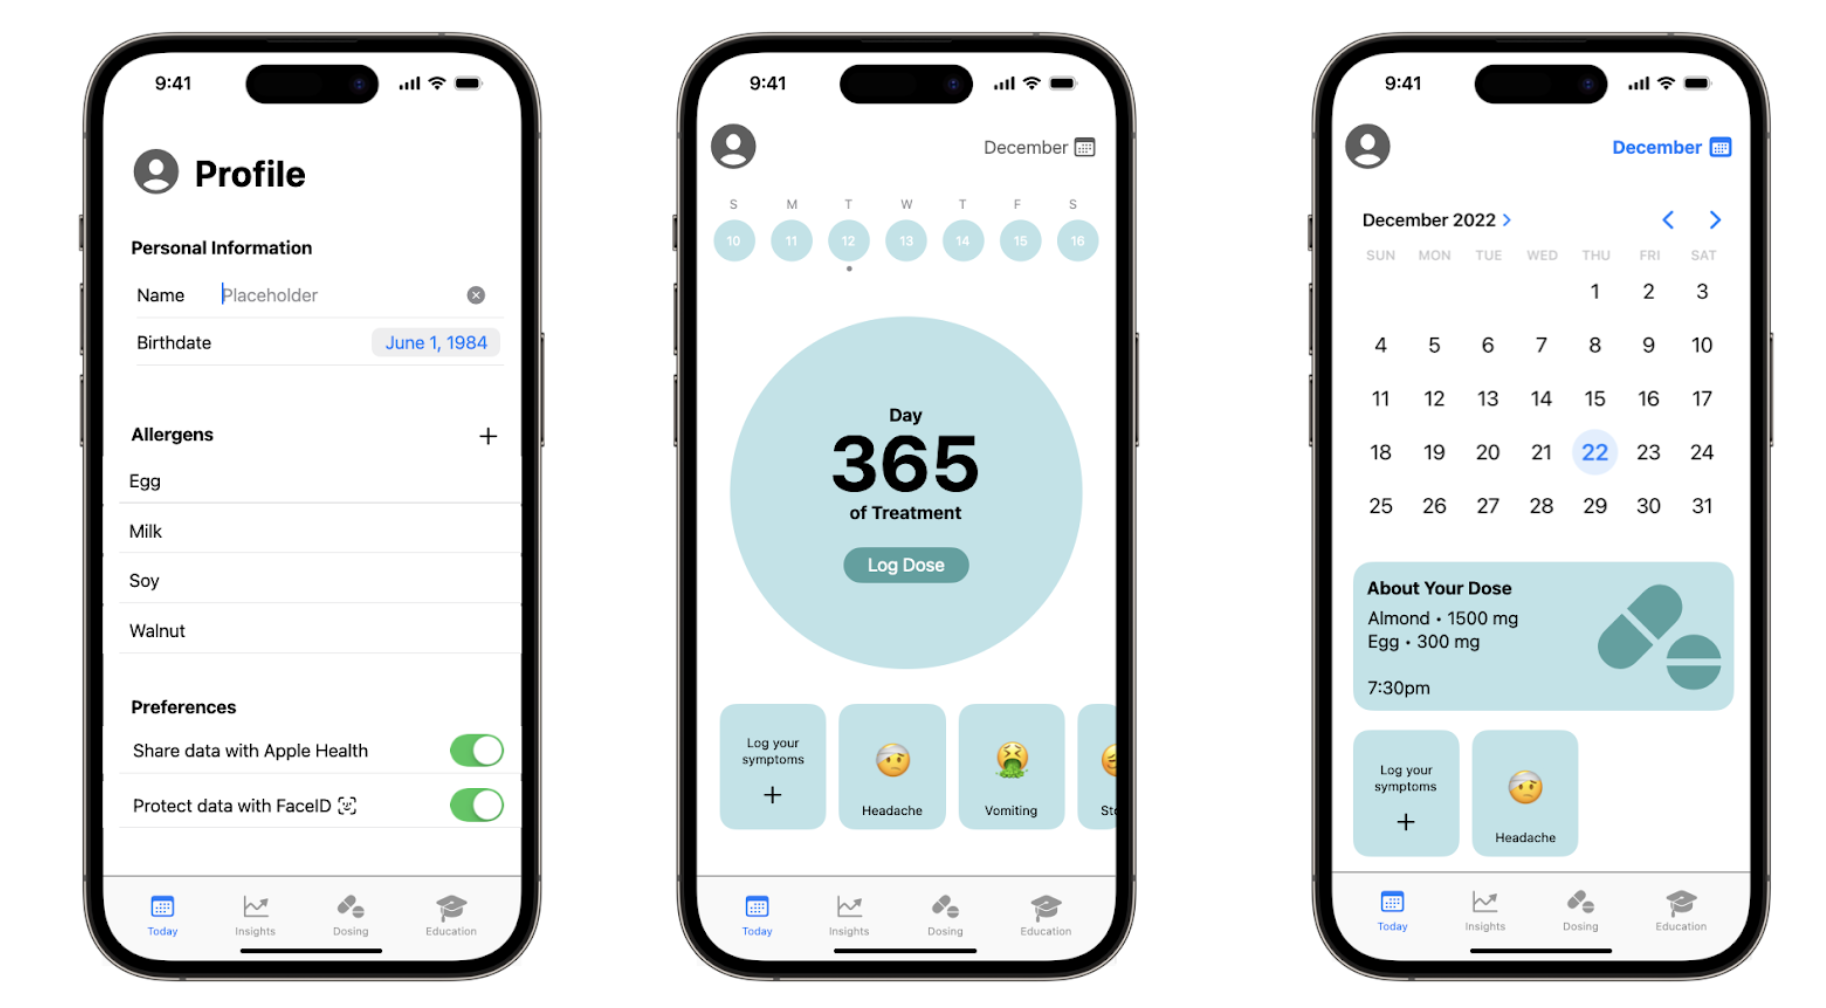
\includegraphics[width=.7\linewidth]{thesis//chapters//images/todayTabScreens.png}
    \caption{Today Tab Screens}
    \label{fig:today-tab-screens}
\end{figure}

\section{Dose and Symptom Pop-Ups}

The Dose and Symptom Pop-Ups, shown in Figure \ref{fig:dose-and-symptom-pop-ups}, are opened when the user goes to log a dose or symptom in the Today tab. These pop-ups are designed to be user-friendly, with helpful graphics, and to make it take minimal time to log a dose or symptom.

In addition to allergens and dosages, the Dosing Pop-Up will collect other important information, such as time of dose and whether the patient has pre-dosed with any medications. And, the symptoms listed in the Symptoms Pop-Up will directly correlate with HealthKit symptom types to ensure ease of Health App reporting.

\begin{figure}[H]
    \centering
    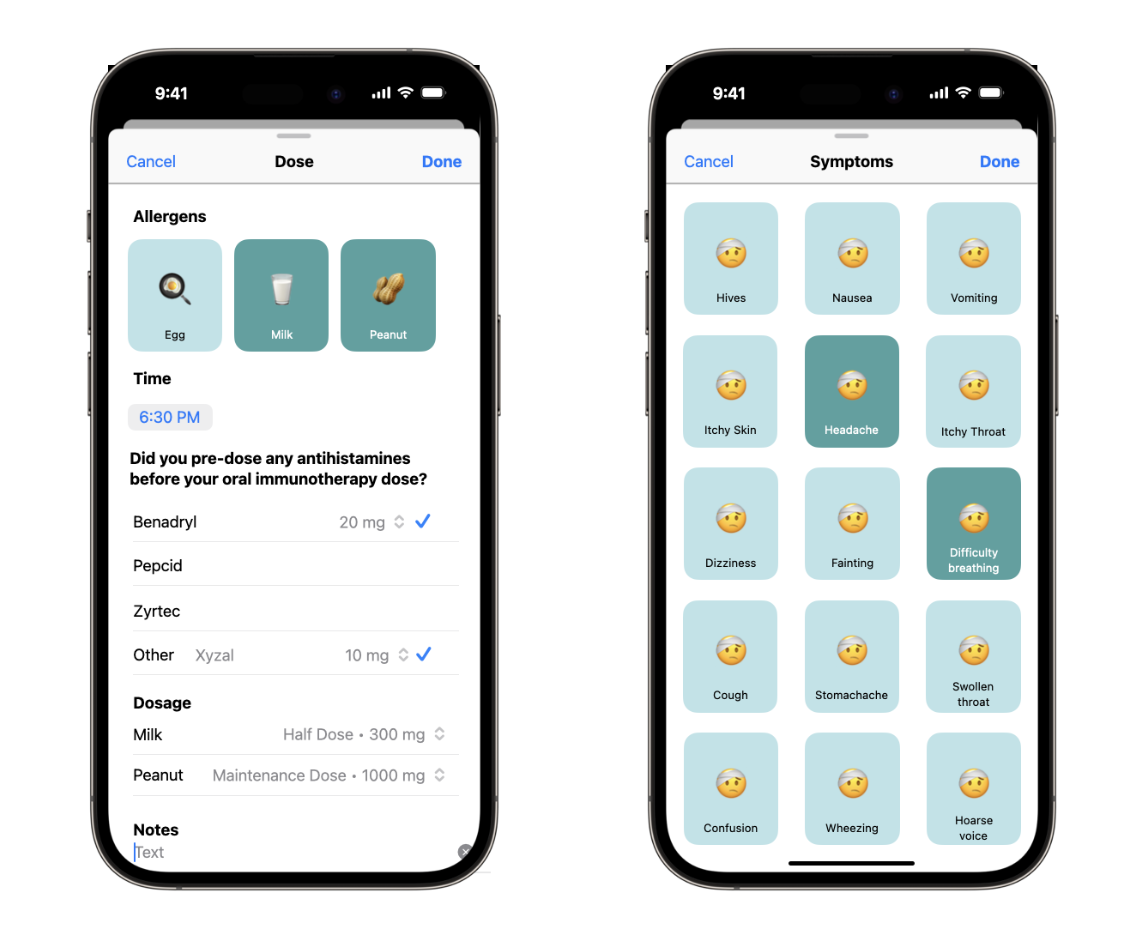
\includegraphics[width=0.5\linewidth]{thesis//chapters//images/doseAndSymptomPopUps.png}
    \caption{Dose and Symptoms Pop-Ups}
    \label{fig:dose-and-symptom-pop-ups}
\end{figure}

\section{Insights Tab}

The Insights Tab, shown in Figure \ref{fig:insights-tab}, serves as a place for the user to view any trends identified by their symptom and dose data, in conjunction with their other Apple Health data. Leveraging SwiftCharts and CareKit, this tab of the application will display these trends in easy-to-interpret ways.

\begin{figure}[H]
    \centering
    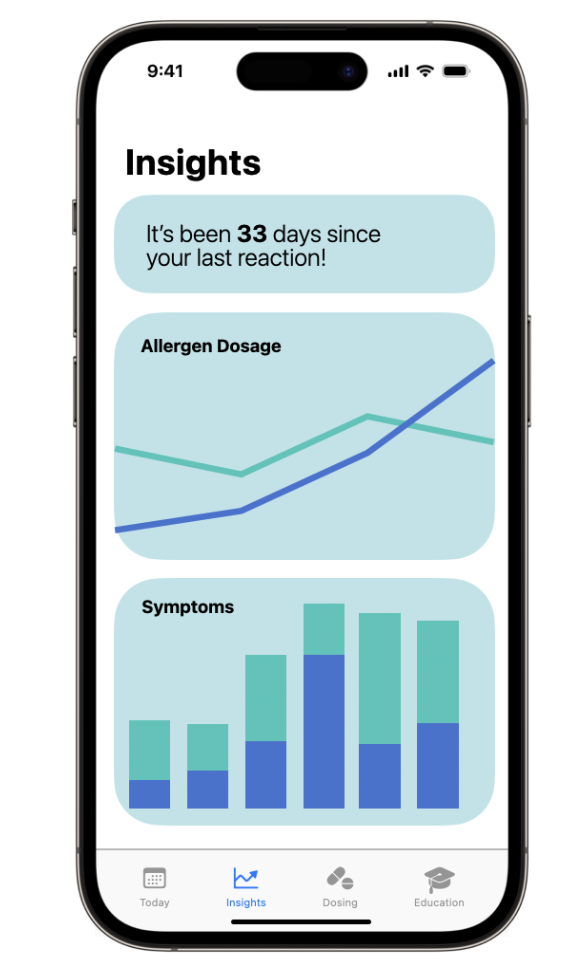
\includegraphics[width=0.25\linewidth]{thesis//chapters//images/insightsTab.png}
    \caption{Insights Tab}
    \label{fig:insights-tab}
\end{figure}

\section{Dosing Tab}

The Dosing Tab, shown in Figure \ref{fig:dosing-tab}, is a place where users can log new dosages of their allergens. The application will store all of the dosages in this tab, as well as calculate half doses for the user, as OIT patients are frequently advised to take half doses when they are sick, traveling, stressed, or in other circumstances that may cause issues with a full dose.

\begin{figure}[H]
    \centering
    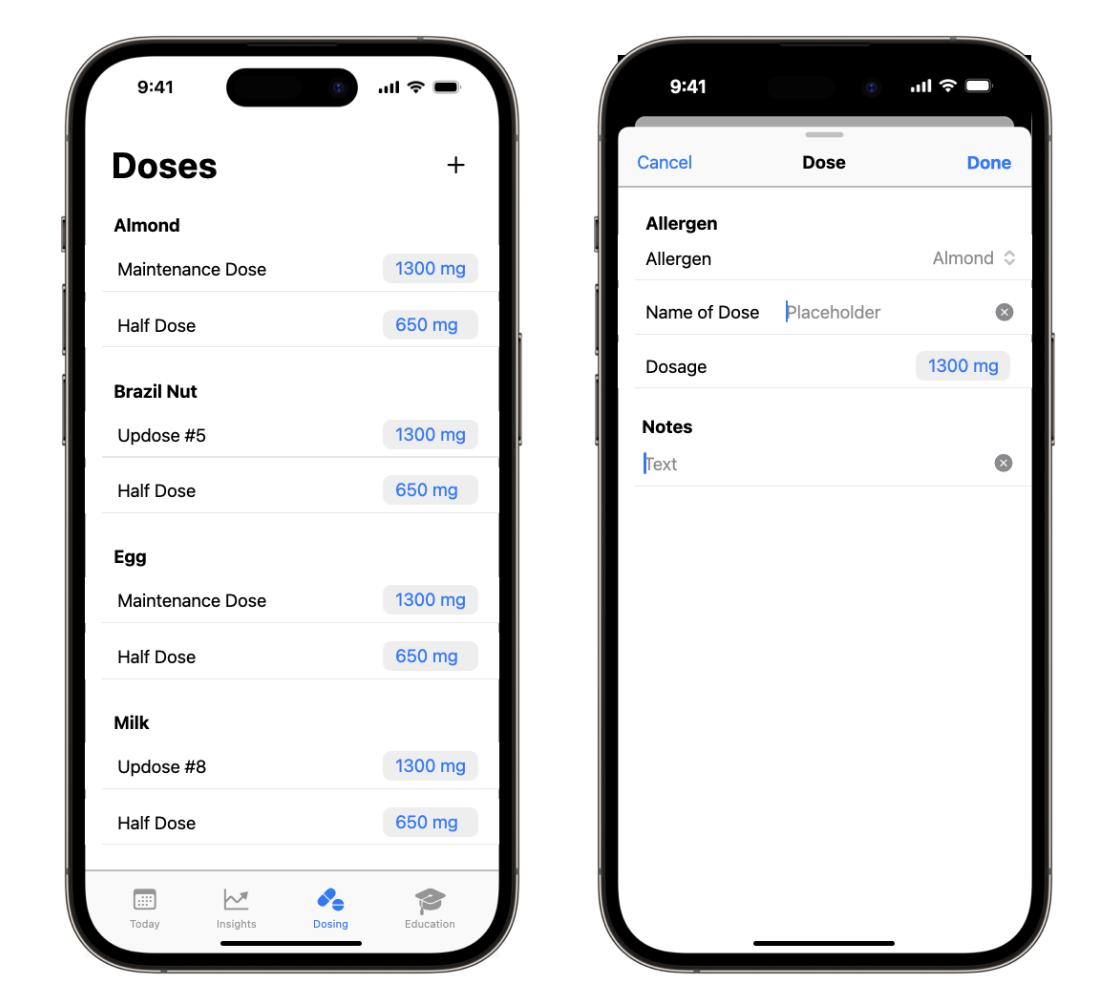
\includegraphics[width=0.45\linewidth]{thesis//chapters//images/dosingTabScreens.png}
    \caption{Dosing Tab Screens}
    \label{fig:dosing-tab}
\end{figure}

\section{Education Tab}

The Education Tab, shown in Figure \ref{fig:education-tab}, is a dedicated space within the application, offering users a wealth of valuable knowledge and resources. This section is thoughtfully curated to provide a comprehensive educational experience, aiming to empower users with essential information related to oral immunotherapy, anaphylaxis, and other pertinent topics. Through a collection of articles and informative resources, the Education Tab serves as an invaluable repository for users seeking to enhance their understanding of the complexities associated with food allergies and the oral immunotherapy process, enabling users to make informed decisions about their health and well-being.

\begin{figure}[H]
    \centering
    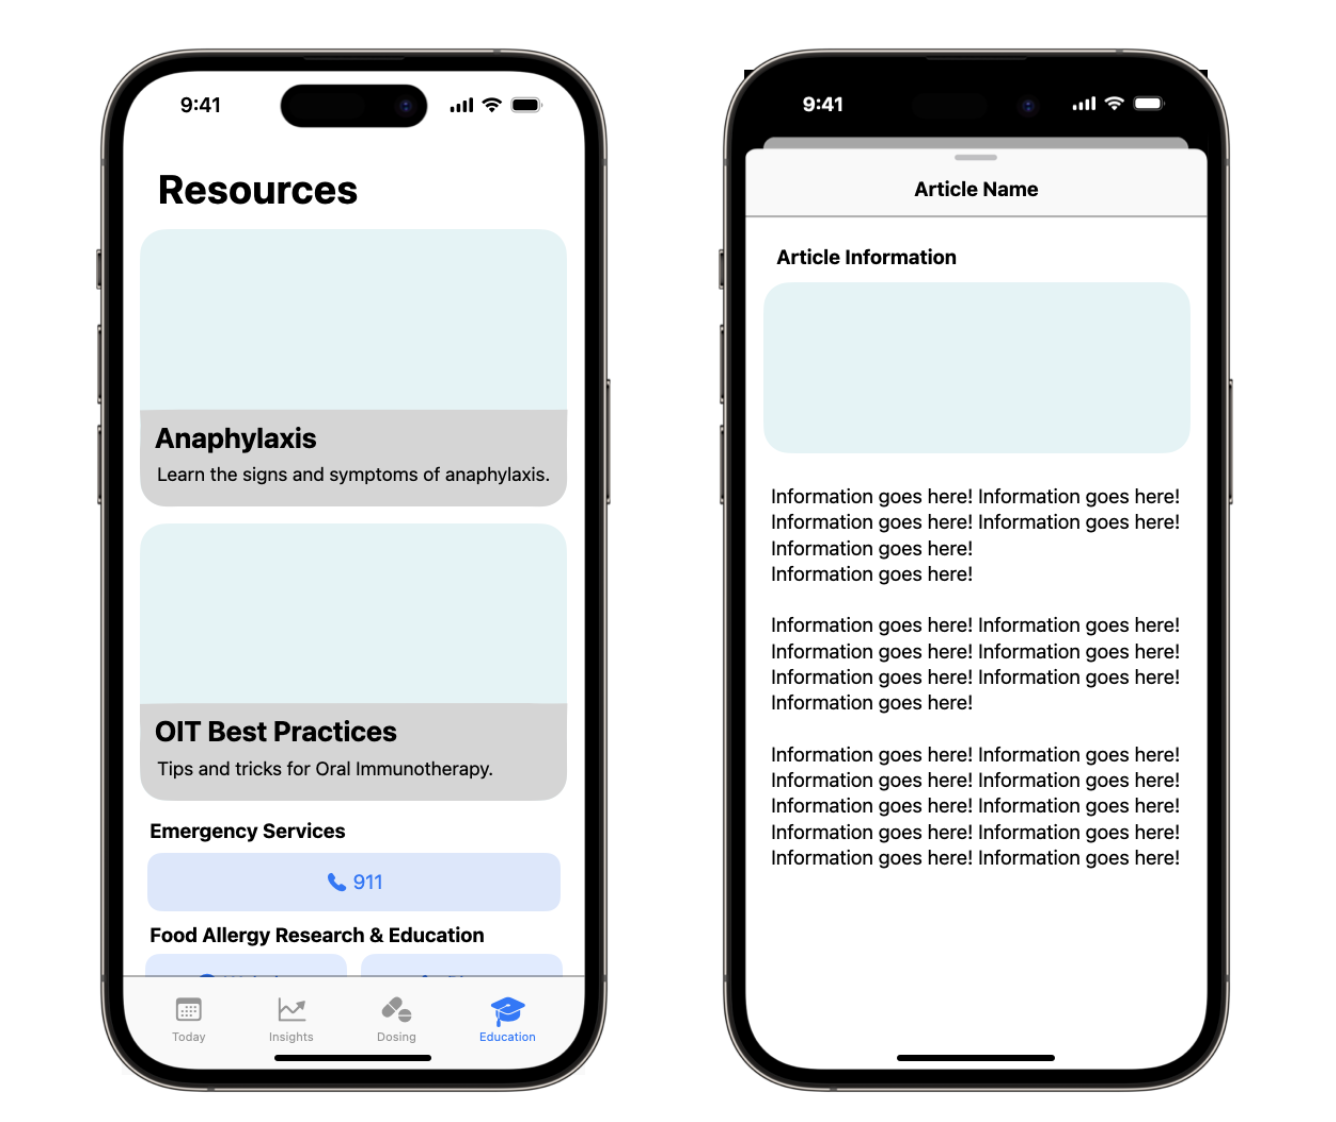
\includegraphics[width=0.5\linewidth]{thesis//chapters//images/education-tab-screens.png}
    \caption{Education Tab Screens}
    \label{fig:education-tab}
\end{figure}

